\documentclass[a4,11pt]{pssbmac}

\usepackage[brazil]{babel}      % para texto em Português
%\usepackage[english]{babel}    % para texto em Inglês

%\usepackage[latin1]{inputenc}   % para acentuação em Português OU
\usepackage[utf8]{inputenc}   % para acentuação em Português com o uso do Unicode, 
% mude a codificação desse padrão para utf-8

%%
%% POR FAVOR, NÃO FAÇA MUDANÇAS NESSE PADRÃO QUE ACARRETEM  EM
%% ALTERAÇÃO NA FORMATAÇÃO FINAL DO TEXTO
%%
\usepackage{graphics}
\usepackage{subfigure}
\usepackage{graphicx}
\usepackage{epsfig}
\usepackage[centertags]{amsmath}
\usepackage{graphicx,indentfirst,amsmath,amsfonts,amssymb,amsthm,newlfont}
\usepackage{longtable}
\usepackage{cite}
\usepackage[usenames,dvipsnames]{color}
\usepackage{booktabs}
\begin{document}
	
	%********************************************************
	\title{Um estudo teórico-computacional da aplicação da Geometria de Distâncias no problema de conformação proteica}
	
	\author{
		{\large Guilherme Philippi}\thanks{guilherme.philippi@hotmail.com}\\
		{\small UFSC, Blumenau, SC} \\
		{\large Felipe Fidalgo}\thanks{felipe.fidalgo@ufsc.br} \\
		{\small MAT/UFSC, Blumenau, SC} \\
	}
	\criartitulo
	
	A Geometria de Distâncias originou-se dos esforços de Menger (1928), seguido por Blumenthal (1953), na caracterização de vários conceitos geométricos (como congruência e convexidade de conjuntos) em termos de distâncias \cite{carlileGDandAplications}. Isso permitiu a formulação do \textit{Distance Geometry Problem} (DGP), conhecido como problema fundamental de Geometria de Distâncias. Trata-se de um problema inverso, onde, dado um grafo simples, ponderado positivamente e não direcionado $G=(V,E, d)$, e um inteiro $k>0$, deseja-se encontrar uma função $x:V\rightarrow\mathbb{R}^k$ (dita realização de $G$ em $\mathbb{R}^k$) tal que $\forall$ $\{u,v\} \in E$, $||x(u) - x(v)|| = d(\{u,v\})$. 
	
	Em particular, é de interesse prático uma restrição desse problema. Trata-se do DGP com $k = 3$, chamado de \textit{Molecular Distance Geometry Problem} (MDGP) --- carrega o termo \textit{molecular} pois, mesmo que não seja exclusivo para essa aplicação \cite{carlileGDandAplications}, teve sua origem associada as estruturas moleculares. Supondo que o conjunto solução de um MDGP seja não vazio, sabe-se que ele é não enumerável ou finito \cite{carlileBook31Coloquio}. A busca pela segunda possibilidade está associada ao conceito de \textit{ordem nos vértices} do grafo $G$ do MDGP (a procura por essa ordem é caracterizado como \textit{Discretization Vertex Order Problem}, ou, DVOP). Munido de tal ordem, o MDGP pode ser discretizado, gerando o problema principal desse trabalho, como segue formalmente definido \cite{carlileBook31Coloquio} \cite{carlileDMDGP}:
	\\
	
	\textbf{Discretizable Molecular Distance Geometry Problem (DMDGP): }Dados um grafo simples, ponderado e não-direcionado $G = (V,E,d)$, onde $d: E \rightarrow \mathbb{R}_{+}$, o subconjunto de vértices $U_{0} = \{v_{1},v_{2},v_{3} \}$ e uma relação de ordem total $v_1, \dots, v_{|V|} \in V$, que satisfaça as propriedades
	\begin{enumerate}
		\item $U_{0}$ é um 3-clique em $G$;
		\vspace{-0.6cm}
		\item 
		\begin{minipage}{0.4\linewidth}  
			$\forall$ $v_{i} \in V$ tal que $i > 3$ nessa ordem:
		\end{minipage}
		\begin{minipage}{0.6\linewidth}
			\vspace{0.6cm}
			-- $U_{i} = \{v_i, v_{i-1}, v_{i-2}, v_{i-3}\}$ é um 4-clique em $G$;
			\vspace{0.2cm}
			
			-- vale a desigualdade $d_{i-3,i-1} < d_{i-3,i-2} + d_{i-2,i-1}$,
		\end{minipage}
		
	\end{enumerate}
	encontre uma realização $x: V \rightarrow \mathbb{R}^{3}$ tal que valha, $\forall$ $\{u,v\} \in E$, $\left\| x(u) - x(v) \right\| = d(\{u,v\})$.
	\\
	
	A ordenação no DMDGP garante, de fato, a finitude do conjunto solução do problema \cite{carlileBook31Coloquio}. Além disso, ela organiza o espaço onde devemos fazer a busca por uma solução. Na verdade, a ordem induz uma estrutura de \textit{árvore binária} no espaço de busca \cite{fidalgotese}. Isto é, a partir do quarto, sempre temos duas possibilidades para a realização de um vértice \cite{carlileDMDGP}. Analisando essa estrutura propuseram um algorítimo chamado \textit{Branch-and-Prune} (BP), que consiste em uma estratégia numérica recursiva para resolver o DMDGP eficientemente, utilizando uma busca combinatória no espaço de busca por soluções. Nele, realiza-se vértice por vértice do grafo, seguindo a ordenação definida pelo DMDGP, ``podando'' (descartando) todo sub-conjunto solução do problema onde uma realização $x(v)$ não respeita ao menos uma das distâncias $d(\{u,v\})$ definidas pelo grafo, isto é, $\left\| x(u) - x(v) \right\| \neq d(\{u,v\})$. Desde que esse algoritmo foi publicado, tem se verificado tanto sua beleza matemática quanto a sua eficiência numérica-computacional para resolver problemas em Geometria de Distâncias \cite{fidalgotese}. 
	
	Especificamente, neste trabalho, buscou-se usar a Geometria de Distâncias como modelo na conformação molecular de proteínas (existe uma relação muito forte com a forma geométrica das moléculas e suas funções em organismos vivos \cite{bioquimicaLehninger}, donde a importância do tema), em conjunto com a interpretação de dados de \textit{Ressonância Magnética Nuclear} (RMN) --- experimentos que tem como resultado distâncias entre alguns átomos próximos na molécula. Esse é um problema inverso, onde possuímos uma série de distâncias e ângulos e queremos descobrir suas posições. Logo, estamos interessados em uma função de realização no espaço $\mathbb{R}^3$, descrita pelo MDGP. Mais do que isso, na verdade, estamos interessados em definir uma ordenação nos átomos da molécula (vértices do grafo), obedecendo a definição do DMDGP, de forma a discretizar o problema.
	
	\begin{figure}[h!]
		\centering
		\begin{minipage}{0.46\linewidth}   
			\paragraph{} Por sorte, essa ordenação já foi proposta em \cite{carlile:MinimalOrder}, pelos mesmo grupo que propôs o algoritmo BP. propondo o \textit{hand-crafted vertex order}, conforme esboça a Figura ~\ref{fig:hcVO} (extraída do texto original). 
		\end{minipage}
		\begin{minipage}{0.532\linewidth}
			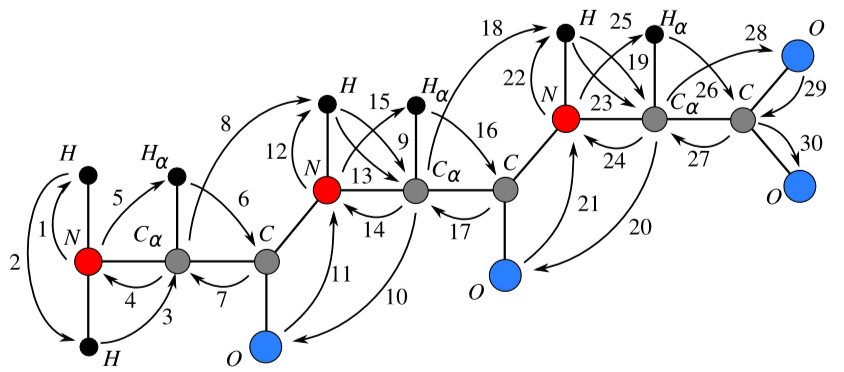
\includegraphics[scale=0.6]{hcVO.png}
			\caption{A ordenação hc.}
			\label{fig:hcVO}
		\end{minipage}
	\end{figure}
	
	\section*{Agradecimentos}
	O presente trabalho foi realizado com o apoio do Conselho Nacional de Desenvolvimento Científico e Tecnológico – CNPq – Brasil. Agradeço a Família, ao Felipão e a organização que prorrogou o período de submissão.
	
	\begin{thebibliography}{00}
		
		\bibitem{fidalgotese}
		Fidalgo, F. Dividindo e conquistando com simetrias em geometria de distâncias. Tese de Doutorado, IMECC/UNICAMP, Campinas - SP, 2015.
		
		\bibitem{carlileBook31Coloquio} 
		Lavor, C., Maculan, N., Souza, M. and Alves, R. {\it Álgebra e Geometria no Cálculo de Estrutura Molecular, 31º Colóquio Brasileiro de Matemática}. IMPA, Rio de Janeiro - RJ, 2017.
		
		\bibitem{carlileDMDGP} 
		Lavor, C., Liberti, L., Maculan, N., and Mucherino, A. The discretizable molecular distance geometry problem, {\it Computational Optimization and Application}, Springer,  volume 52, number 1, pages 115-146, 2012. DOI. 10.1007/s10589-011-9402-6.
		
		\bibitem{carlile:MinimalOrder}
		Lavor, C., Liberti, L., Donald, B., Worley, B., Bardiaux, B., Malliavin, T. E. and Nilges, M. Minimal NMR distance information for rigidity of protein graphs, {\it Discrete Applied Mathematics}, Elsevier, 256:91--104, 2019. DOI:10.1016/j.dam.2018.03.071.
		
		\bibitem{carlileGDandAplications} 
		Liberti, L., Lavor, C., Maculan, N. and Mucherino, A. Euclidean distance geometry and applications, {\it SIAM REVIEW}, Society for Industrial and Applied Mathematics,  volume 56, number 1, pages 3-69, 2014. DOI. 10.1137/120875909.
		
		\bibitem{bioquimicaLehninger} 
		Nelson, D. L. and Cox, M. M. {\it Lehninger principles of biochemistry, 6th edition}.  W.H.Freeman and Company, New York, 2012.
		
		
		%\bibitem{Boldrini} 
		%Boldrini, J. L., Costa, S. I. R., Ribeiro, V. R. and Wetzler, H. G. {\it Álgebra Linear e Aplicações, 3a. edição}. Harbra, São Paulo, 1984.
		%
		%\bibitem{Cuminato}
		%Cuminato, J. A. and Ruas, V. Unification of distance inequalities for linear variational problems, 
		%{\it Comp. Appl. Math.}, 2014. DOI: 10.1007/s40314-014-0163-6.
		%
		%\bibitem{daSilva} 
		%Da Silva, P. L. and Freire, I. L. On the group analysis of a modified Novikov equation, 
		%{\it Interdisciplinary Topics in Applied Mathematics, Modeling and Computational Science}, 
		%Springer Proceedings in Mathematics and Statistics,  volume 117, chapter 23, pages 161-166, 2015.
		%
		%\bibitem{Diniz1}
		%Diniz, G. L. A mudança no habitat de populações de peixes: de rio a represa -- o modelo 
		%matemático, Dissertação de Mestrado, Unicamp, 1994.
		%
		%\bibitem{Diniz2}
		%Diniz, G. L., Meyer, J. F. C. A. e Barros, L. C. Solução numérica para um problema de 
		%Cauchy Fuzzy que modela o decaimento radioativo, {\it TEMA},  23:63--72, 2001. DOI:10.1007/s40314-014-0163-6.
		%
		%\bibitem{Gomes}
		%Gomes, L. T., De Barros, L. C. and Bede, B. Fuzzy differential equation in various approaches. 
		%In {\it SpringerBriefs in Mathematics}. SBMAC- Springer, 2015. ISSN: 2191-8198.
		%
		%\bibitem{Jafelice} Jafelice, R. M., Barros, L. C. and Bassanezi, R. C. Study of the dynamics of HIV under treatment considering fuzzy delay, {\it Comp. Appl. Math.}, 33:45--61, 2014.
		
		%\bibitem{Mallet}
		%Mallet, S. M. Análise Numérica de Elementos Finitos. Tese de Doutorado, LNCC/MCTI, 1990.
		
		%\bibitem{Santos} Santos, I. L. D. e Silva, G. N. Uma classe de problemas de controle ótimo 
		%em escalas temporais, {\it Proceeding Series of the Brazilian Society of Computational and 
		%	Applied Mathematics}, volume 1, 2013. DOI: 10.5540/03.2013.001.01.0177.
		
	\end{thebibliography}
\end{document}